\documentclass[a4paper,11pt]{article}
\RequirePackage[T1]{fontenc}

\usepackage{times}
\usepackage{calc}
\usepackage[shortcuts]{extdash}
\usepackage{graphicx}

\usepackage{natbib}
\usepackage{hyperref}
\usepackage{doi}
\usepackage{bibentry}

\reversemarginpar

\usepackage[paper=letterpaper,
            marginparwidth=1.1in,     % Length of section titles
            marginparsep=.075in,      % Space between titles and text
            margin=0.5in,             % 1 inch margins
            tmargin=0.65in,
            includemp]{geometry}

\setlength{\parindent}{0in}

\usepackage{fancyhdr,lastpage}
\pagestyle{fancy}
%\pagestyle{empty}      % Uncomment this to get rid of page numbers
\fancyhf{}\renewcommand{\headrulewidth}{0pt}
\fancyfootoffset{\marginparsep+\marginparwidth}
\newlength{\footpageshift}
\setlength{\footpageshift}
          {0.5\textwidth+0.5\marginparsep+0.5\marginparwidth-2in}
\lfoot{\hspace{\footpageshift}%
       \parbox{4in}{\, \hfill %
                    \arabic{page} of \protect\pageref*{LastPage} % +LP
%                    \arabic{page}                               % -LP
                    \hfill \,}}

\usepackage{xcolor}
\definecolor{darkblue}{rgb}{0.0,0.0,0.3}
\hypersetup{colorlinks,breaklinks,
            linkcolor=darkblue,urlcolor=darkblue,
            anchorcolor=darkblue,citecolor=darkblue}

\renewcommand{\section}[1]{\pagebreak[3]%
    \vspace{1.3\baselineskip}%
    \phantomsection\addcontentsline{toc}{section}{#1}%
    \noindent\llap{\scshape\smash{\parbox[t]{\marginparwidth}{\hyphenpenalty=10000\raggedright #1}}}%
    \vspace{-\baselineskip}\par}

\usepackage{url}

\urlstyle{same}

\definecolor{dimmedgrey}{rgb}{0.5,0.5,0.5}
\newcommand{\dimmed}[1]{\textcolor{dimmedgrey}{#1}}

\newenvironment{tightitemize}
{ \begin{itemize}
  \setlength{\itemsep}{0pt}
  \setlength{\parskip}{0pt}
  \setlength{\parsep}{0pt}
    \vspace{-0.5cm}}
{ \end{itemize} }

\begin{document}

 {\hspace*{-\marginparsep minus \marginparwidth}%
\begin{minipage}[t]{\textwidth+\marginparwidth+\marginparsep}%
  {\LARGE \bfseries {Patrick Sanan}}\hfill \dimmed{Curriculum Vit\ae}\\
\vspace{0.2cm}
\rule{\columnwidth}{1.2pt}
\end{minipage}}

\begin{minipage}{0.75\textwidth}
\section{Contact}
\begin{minipage}{0.49\textwidth}
\href{mailto:patrick.sanan@gmail.com}{patrick@patricksanan.org} \\
\href{https://patricksanan.org}{patricksanan.org}\\
%+41 77 485 17 96 \dimmed{(mobile)}%\\
%+41 44 632 02 44 \dimmed{(office)}
\end{minipage}
\begin{minipage}{0.5\textwidth}
Institute of  Geophysics\\
Sonneggstrasse 5\\
ETH Zurich, NO H 9.3\\
8092 Zurich, Switzerland
\end{minipage}

\section{Citizenship}
Ireland, United States
\vspace{-0.6cm}

\section{Residency}
Switzerland \dimmed{(Zurich, C)}
\vspace{-0.6cm}

\section{Languages}
English \dimmed{(native)}, German \dimmed{(B2)}

\end{minipage}
\begin{minipage}{0.25\textwidth}
  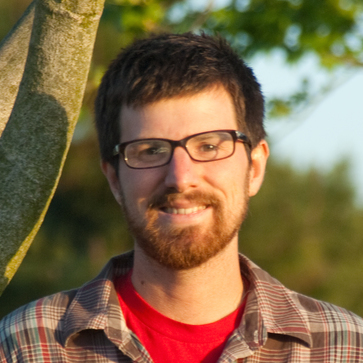
\includegraphics[width=\textwidth]{portrait.jpg}
\end{minipage}


 {\hspace*{-\marginparsep minus \marginparwidth}%
\begin{minipage}[t]{\textwidth+\marginparwidth+\marginparsep}%
\vspace{0.2cm}
\rule{\columnwidth}{1.2pt}
\end{minipage}}

\vspace{0.2cm}

\section{Profile}

Applied mathematician, computational scientist, and software developer, with expertise in scientific software (in particular with the PETSc library), scalable algorithms, high performance computing, linear algebra, numerical PDEs, finite element methods, computational geometry, computational earth science, sound and music generation.

\vspace{0.2cm}

\section{Technical Skills}
\dimmed{very experienced:} C, C++, Python, Git, shell scripting, MPI, MATLAB, \LaTeX \\
\dimmed{significant experience:} Fortran, CUDA, Cray systems, OpenMP, Mathematica, Julia
%\textbf{HPC Systems}: Cray \\
%\textbf{Animation/FX Software} : Houdini \\
%\textbf{CAD Software}: Pro/Engineer, AutoCAD, Inventor\\
%\textbf{Audio Software}: ProTools, Logic, Digital Performer, MAX/MSP, Pd, SuperCollider\\
% Processing

% FIXME: add software section
% - PETSc (make sure to note docs contributions..)

\section{Education}

\textbf{Ph.D. Applied and Computational Mathematics},
\href{https://caltech.edu}{California Institute of Technology (Caltech)}
\hfill {2013}

\vspace{0.2cm}
\textbf{MusM Electroacoustic Music Composition},
\href{https://www.manchester.ac.uk/}{University of Manchester}
\hfill {2007}\\
With Distinction

\vspace{0.2cm}
\textbf{B.S. Aerospace Engineering}\\
\textbf{B.A. Math-Applied Science},
\href{https://ucsd.edu}{University of California, San Diego (UCSD)} \hfill {2006}\\
Minor: Music \\
%La Jolla, California, United States\\
Summa Cum Laude\\
%GPA: 3.95, 3.98 Major
%GPA: 3.95 Cum., 3.98 Major, 3.99 last two years, 3.98 upper div\\

%\vspace{0.1cm}
%\textbf{Diploma}
%\href{https://www.acalanes.k12.ca.us/laslomas}{Las Lomas High School}
%\hfill{2002}
%%Walnut Creek, California, United States
%%GPA: 4.5, Graduation with Honors

\section{Professional Experience}

\textbf{Computational Mathematician},
Argonne National Laboratory
\hfill {November 2021--Present}\\
Remote contractor \\
\href{https://www.anl.gov/mcs/lans}{Laboratory for Applied Mathematics, Numerical Software, and Statistics}\\

\textbf{Scientific Collaborator}, \textbf{Lecturer},
ETH Zurich
\hfill {November 2021--Present}\\
\href{https://www.pasc-ch.org/projects/2021-2024/gpu4geo/}{PASC \textsc{GPU4GEO} Software Development Project} \\
\href{https://gfd.ethz.ch/}{Geophysical Fluid Dynamics Group}\\
{\small
PI: Paul J. Tackley \\
}

\textbf{Postdoctoral Researcher}, \textbf{Lecturer},
ETH Zurich
\hfill {July 2021--October 2021}\\
\href{https://www.pasc-ch.org/projects/2021-2024/gpu4geo/}{PASC \textsc{GPU4GEO} Software Development Project} \\
\href{https://gfd.ethz.ch/}{Geophysical Fluid Dynamics Group}\\
{\small
PI: Paul J. Tackley \\
}

\textbf{Postdoctoral Researcher}, \textbf{Lecturer},
ETH Zurich
\hfill {November 2017--June 2021}\\
\href{https://www.pasc-ch.org/projects/2017-2020/stagbl/}{PASC \textsc{StagBL} Software Development Project} \\
\href{https://gfd.ethz.ch/}{Geophysical Fluid Dynamics Group}\\
{\small
PI: Paul J. Tackley \\
\begin{tightitemize}
  \item Led development on \href{https://github.com/stagbl/stagbl}{\textsc{StagBL}}, \texttt{DMStag} within \textsc{PETSc}, and \href{https://github.com/sciath/sciath}{\textsc{SciATH}}
\item Collaborated on several publications on Earth and Planetary science, as well as on solvers.
\end{tightitemize}
}

\textbf{Postdoctoral Researcher},
ETH Zurich
\hfill {October 2017}\\
\textsc{SALVUS} Project\\
\href{https://geophysics.ethz.ch/research/groups/swp.html}{Seismology and Wave Physics Group}\\
{\small
%PI: Andreas Fichtner \\
\begin{tightitemize}
  \item Performed initial investigations into accelerating use of \textsc{PETSc}'s DMPlex within \textsc{SALVUS}.
\end{tightitemize}
}

\textbf{Postdoctoral Researcher},
Universit\'{a} della Svizzera italiana (USI)
\hfill {June 2014--September 2017} \\
\href{http://www.pasc-ch.org/projects/projects/geopc/}{PASC GeoPC Co-Design Project} \\
{\small
PI: Paul J. Tackley (ETH Zurich) \\
Advisors: Olaf Schenk (USI), Dave A. May (ETH Zurich) \\
\begin{tightitemize}
\item Researched and implemented large-scale, parallel, communication-avoiding and GPU-accelerated operators and multigrid smoothers for large-scale Stokes flow.
\end{tightitemize}
}

\textbf{Givens Scholar},
\href{http://www.mcs.anl.gov}{MCS Division, Argonne National Laboratory}
\hfill {Summer 2013}\\
Supervisor: \href{https://jedbrown.org/}{Jed Brown} \\
%Lemont, IL, United States
{\small
\begin{tightitemize}
\item Investigated multiscale integrators in \textsc{PETSc}
\end{tightitemize}
}

\textbf{Software Engineering Intern},
\href{http://www.rhythm.com}{Rhythm and Hues Studios}
\hfill {Summer 2012}\\
El Segundo, CA, United States \\
{\small
\begin{tightitemize}
\item Worked with the software engineering team at an award-winning (Babe, Life of Pi, etc.) graphics studio.
\item Researched and implemented a surface parameterization algorithm minimizing an elastic energy under inversion constraints.
\end{tightitemize}
}

\textbf{Teaching Assistant and Instructor},
Caltech
\hfill {Fall--Spring 2008-2013\\
%Applied and Computational Mathematics, Caltech \\
% Served as instructor for a course on MATLAB/Mathematica, and served as Teaching Assistant for many courses.

\textbf{Grader and Tutor},
UCSD
\hfill{Fall 2004, Summer 2005}\\
%\textbf{Grader}
%\hfill {Summer 2005}\\
% MAE 101B: Advanced Fluid Dynamics, UCSD\\
%
%\textbf{Tutor}
%\hfill {Fall 2004}\\
% MAE 3: Introduction to Design and Graphics, UCSD\\

\textbf{Mechanical Engineering Intern},
General Atomics Lynx Systems
 \hfill {Summer 2004}\\
San Diego, CA, United States \\
% Description:
{\small
\begin{tightitemize}
\item Performed CAD and analysis for synthetic aperture radar.
\end{tightitemize}
}

\textbf{Sales Clerk}, Long Drugs \hfill {part time 2000-2001}\\
Walnut Creek, CA, United States
% Cashier, stocking, customer service, ice cream scooping.

\section{Publications}
\bibliographystyle{plainnat}
\nobibliography{pds.bib}
{
  \newcommand{\publication}[1]{$\bullet$ \bibentry{#1}\vspace{5pt}\\}
  % Want SananMay SciATH preprint here!!
  % Want SananEtAl DMStag preprint here!!
  % Want SananEtAl AMR preprint here!!
  % SananTurner2019 resub ?
  \publication{PrangerEtAl2022}
  \publication{BowerHakimSossiSanan2021}
  \publication{AdamsEtAl2022}
  \publication{SunEtAl2021}
  \publication{BolraoEtAl2021}
  \publication{LichtenbergEtAl2021}
  \publication{MorganSananKnepleyMills2020}
  \publication{RibeTackleySanan2020}
  \publication{SananMayBollhoeferSchenk2020}
  \publication{BowerEtAl2019}
  \publication{JainEtAl2019}
  \publication{KrugerSananSmith2018}
  \publication{DonfackEtAl2018}
  \publication{BowerSananWolf2018}
  \publication{BalayEtAl2017b}
  \publication{MayEtAl2016}
  \publication{SananSchneppMay2016}
  \publication{MorganKnepleySananScott2016}
  \publication{Sanan2014}  % Include link to goofy video from UCSD?
  \publication{ChaoPinkallSananSchroeder2010}
  %Patrick Sanan and Nathan Litke, ``Bounded-distortion Surface Parameterization with Seam Constraints'', 2013 [preprint, included in thesis]
  %Patrick Sanan and Peter Schr\"{o}der, ``Logarithmic Strain Measures for Elasticity Simulation and Geometry Processing'', 2012 [preprint, included in thesis]
  %Wang-Juh Chen, Hoi Tin Kong, Minah Oh, Patrick Sanan, Ying Wang and Brendt Wohlberg.``Visual Words: Text Analysis Concepts for Computer Vision'', 2009 [preprint; Part of an IMA team workshop]. %https://www.ima.umn.edu/Visual-words-text-analysis-concepts-computer-vision
}

\section{Selected Talks}
% EGU 2021 great debate: https://great-debate-research-software.github.io/
{
  \newcommand{\talk}[1]{$\bullet$ #1\vspace{5pt}\\}
  \talk{``Performance-Portable Staggered Grid Stokes Flow Solves with StagBL and MARS``, SIAM CSE (virtual), March 4, 2021.}
  %\talk{``\textsc{StagBL}: A Scalable, Portable, High-Performance Discretization and Solver Layer for Geodynamic Simulation'', with Paul J. Tackley, PASC Review, January 15, Universit\`{a} della Svizzera italiana, Lugano, Switzerland}
  \talk{``Staggered Grid Abstractions for Scalable Solvers'', FOALAB Group Meeting, University of Oxford, October 18, 2019.}
  \talk{ ``\textsc{StagYY} and \textsc{StagBL}: Developing Tools for Large-Scale Geodynamic Simulations Using Staggered-Grid Discretisation on Hybrid Architectures'', PASC 19 Conference, ETH Zurich, Zurich, Switzerland, June 12-14, 2019.}
  \talk{ ``Modern Solvers for Global Mantle Convection: \textsc{StagYY} with \textsc{StagBL}'' (PICO presentation), EGU General Assembly, Vienna, Austria, April 8-12, 2019.}
  \talk{ ``\textsc{DMStag}: A Staggered-grid Abstraction for \textsc{PETSc}'', \textsc{PETSc} Users' Meeting, Imperial College, London, United Kingdom, June 4-6, 2018.}
  \talk{ ``Hybrid Operators and Composable Software within Lithospheric Dynamic Simulation'', SIAM Conference on Parallel Processing for Scientific Computing, Tokyo, Japan, March 7-10, 2018.}
  \talk{ ``\textsc{StagBL}: A Scalable, Portable, High-Performance Discretization and Solver Layer for Geodynamic Simulation'', PASC 18 Conference, Basel, Switzerland, July 2-4, 2018.}
  \talk{ ``GeoPC: Composable Solvers for Geophysics on Modern Architectures'', PASC 17 Conference, Lugano, Switzerland, June 26-28, 2017. [\href{http://patricksanan.com/talks/SANAN_patrick_PASC17.pdf}{slides online}]}
  \talk{ ``Preconditioners for Stokes Flow with Highly Heterogeneous Viscosity Structure: Saddle-Point Smoothing Via Local Incomplete Factorization'', SIAM CSE, Atlanta, United States, February 27-March 3, 2016.}
  \talk{ ``Robust Multigrid Solvers For Highly Heterogeneous Stokes Flow,'' Swiss Geoscience Meeting, Geneva, Switzerland, November 18-19, 2016.}
  \talk{ ``Robust Multigrid Solvers for Geodynamics,'' German-Swiss Geodynamics Workshop, Lichtenfels, Germany, September 11-14, 2016.}
  \talk{ ``Extreme-scale Multigrid Components within PETSc'', PETSc Users Meeting, Vienna, Austria, June 28-30, 2016.}
  \talk{ ``Extreme-scale Multigrid Components within PETSc'', ACM/PASC16 conference, Lausanne, Switzerland, June 8-10, 2016.[\href{http://insidehpc.com/2016/06/extreme-scale-multigrid/}{video online}]}
  \talk{ ``Accelerating Parallel Multilevel Solvers for Stokes Flow with Highly Heterogeneous Viscosity Structure: Localized Incomplete $LDL^T$ Smoothers and GPUs'', EGU General Assembly, Vienna, Austria, April 17-22, 2016.}
  \talk{ ``Co-designing algorithms: Pipelined, Flexible Krylov Subspace Methods and  Accelerated Subdomain Solves'',  SeisMIC, Technical University of Ostrava, Czech Republic, February 5, 2016.}
  \talk{ ``Co-designing algorithms: Pipelined, Flexible Krylov Subspace Methods and  Accelerated Subdomain Solves'', Computing Sciences Seminar, Lawrence Berkeley Lab, January 12, 2016.}
  \talk{ ``Pipelined, Flexible Krylov Subspace Methods and Accelerated Subdomain Smoothing: Attacks on aggressive nested preconditioners for challenging geophysical Stokes flow problems''[minisymposium talk], SIAM Conference on Applied Linear Algebra, Atlanta, Georgia, USA, October 26-30, 2015.}
  \talk{ ``Towards Aggressive, Accelerated Multigrid Smoothing''[invited talk], ASE Seminar, University of Tokyo, Tokyo, Japan, October 16, 2015.}
  \talk{ ``Pipelined, Flexible Krylov Subspace Methods''[invited talk], IWACOM-III, Tokyo, Japan, October 12-14, 2015.}
  \talk{ ``Using Julia on a Cray Supercomputer''[lightning talk], Juliacon 2015, MIT, Boston, Massachusetts, USA, June 24-27, 2015. [\href{https://www.youtube.com/watch?v=NwyKz2KLdtY}{video online}]}
}

%\section{Posters}
%\begin{tightitemize}
%  \item Patrick Sanan, ``StagBL: A Modern Discretization and Solver Library for Geodynamics'', Ada Lovelace Workshop, Siena, Italy, August 25-30, 2019.
%  \item Patrick Sanan, Paul J. Tackley, Taras Gerya, Boris J.P. Kaus, Dave A. May,``\textsc{StagBL}: A scalable, portable, high-performance discretization and solver layer for geodynamic simulation'', SIAM Conference on Parallel Processing for Scientific Computing, Tokyo, Japan, March 7-10, 2018.
%  \item Patrick Sanan, Paul J. Tackley, Taras Gerya, Boris J.P. Kaus, Dave A. May,``\textsc{StagBL}: A scalable, portable, high-performance discretization and solver layer for geodynamic simulation'', Swiss Geocomputing Center Kickoff Meeting, Lausanne, Switzerland, October 15-17, 2018.
%  \item Patrick Sanan, Paul J. Tackley, Taras Gerya, Boris J.P. Kaus, Dave A. May,``\textsc{StagBL}: A scalable, portable, high-performance discretization and solver layer for geodynamic simulation'', GeoMod 2018, Barcelona, Spain, October 1-4, 2018.
%  \item Patrick Sanan, Paul J. Tackley, Taras Gerya, Boris J.P. Kaus, Dave A. May,``\textsc{StagBL}: A scalable, portable, high-performance discretization and solver layer for geodynamic simulation'', PASC 18, Basel, Switzerland, July 2-4, 2018.
%  \item Patrick Sanan, Paul J. Tackley, Taras Gerya, Boris J.P. Kaus, Dave A. May, ``\textsc{StagBL}: A Parallel Solver and Discretization Library for Geodynamic Simulation on Staggered Grids'', EGU General Assembly, Vienna, Austria, April 23-28, 2018.
%\item Patrick Sanan, Paul J. Tackley, Taras Gerya, Boris J.P. Kaus, Dave A. May,``StagBL: A Scalable, Portable, High-Performance Discretization and Solver Layer for Geodynamic Simulation'', AGU Fall Meeting, December 11-15, 2017, New Orleans, United States.
%\item Patrick Sanan, Paul J. Tackley, Taras Gerya, Boris J.P. Kaus, Dave A. May,``StagBL: A Scalable, Portable, High-Performance Discretization and Solver Layer for Geodynamic Simulation'', Swiss Geoscience Meeting, November 17-18, 2017, Davos, Switzerland.
%\item Patrick Sanan, Dave A. May, Olaf Schenk, Matthias Bollh\"{o}fer, ``Techniques and Software for Monolithic Preconditioning of Moderately-sized Geodynamic Stokes Flow Problems'', EGU General Assembly, April 23-28, 2017, Vienna, Austria.
%\item Patrick Sanan, Olaf Schenk, Dave May, Matthias Bollh\"{o}fer, Karl Rupp, ``Advancing Parallel Multigrid Solvers for Highly Heterogeneous Viscosity Stokes Flow Structure through Localized Incomplete $LDL^T$ Smoothers'' , SIAM Conference on Parallel Processing 2016, April 12-15, Paris, France.
%\item Patrick Sanan, ``Pipelined, Flexible Krylov Methods''[poster, lightning talk], PETSc-20 Conference, June 15-18, Argonne National Laboratory, United States.
%\item Patrick Sanan, Dave A. May, Olaf Schenk, Karl Rupp, ``Aggressive Local Smoothing on Accelerators for Stokes Flow'', PASC 2015, June 1-3, Zurich, Switzerland.
%\item Sascha M. Schnepp, Patrick Sanan, Dave A. May, ``Pipelined Flexible Krylov Subspace Methods for Large-Scale Computing'', PASC 2015, Zurich, Switzerland.
%\item Patrick Sanan, ``Aggressive Accelerator-enabled Local Smoothing via Incomplete Factorization, with Applications'', HPCSE 2015, May 25-28, Ostrava, Czech Republic.
%\item Patrick Sanan, Sascha M. Schnepp, Dave A. May, ``Pipelined, Flexible Krylov Subspace Methods'', EGU General Assembly, April 13-17, 2015, Vienna, Austria
%\item Patrick Sanan, ``Fine-Grained ILU Methods for Aggressive Smoothing in Stokes Preconditioners'', Sparse Solvers for Exascale Workshop, March 23-25, 2015, Greifswald, Germany
%\item Patrick Sanan, Sascha M. Schnepp, Dave A. May, Olaf Schenk, ``Exploring Solver Space for Stokes Flow with Highly Heterogeneous Viscosity Structure'', AGU Fall Meeting 2014, December 15-19, San Francisco, California, United States
%\item Patrick Sanan, ``Exploring Solver Space for Stokes Flow with Highly Heterogeneous Viscosity Structure'', International Symposium on Post-Petascale System Software (ISP2S2), December 2-4, 2014, Kobe, Japan
%\item Patrick Sanan, ``Geometric Elasticity with Applications to Surface Parameterization'', Google LAX PhD Summit 2013 (best poster)
%\item Patrick Sanan, ``Sound Synthesis with Nonlinear Elastodynamics and Fully Variational Integrators", International Computer Music Conference 2011 .
%\end{tightitemize}

%\section{Community Service}
% PASC 22 Scientific / MS+Posters committee
% Have reviewed for X,Y,Z (see reviews directory)
% (Definitely include JOSS if I do a review for them)
% JOSS (Mandyoc: https://doi.org/10.21105/joss.04070)

\section{Teaching}
\textbf{651-4144-00L Introduction to Finite Element Modelling in Geosciences}
\hfill ETH Zurich \\
\textbf{Lecturer}
\href{http://jupiter.ethz.ch/~gfdteaching/femblockcourse/2021/}{[website]}
\hfill {Summer 2018, 2019, 2020, 2021} \\
\textbf{Instructor}
\href{https://jupiter2.ethz.ch/~gfdteaching/femblockcourse/2017/}{[website]}
\hfill {Summer 2017} \\
\textbf{Assistant}
\href{http://jupiter.ethz.ch/~gfdteaching/femblockcourse/2016/}{[website]}
\hfill {Summer 2016}\\

\textbf{HPC Libraries}
\hfill \href{https://cscs.ch}{CSCS} Summer School\\
\textbf{Instructor}
\href{https://github.com/eth-cscs/SummerSchool2017}{[materials online]}
\hfill {July 27, 2017} \\
\textbf{Instructor}
\href{https://github.com/eth-cscs/SummerSchool2016}{[materials online]}
\hfill {July 28, 2016}\\
\textbf{Instructor}
\href{https://github.com/eth-cscs/SummerSchool2015/tree/master/libraries}{[materials online]}
\hfill {August 30, 2015} \\

\textbf{Software Engineering For Computational Science}
\hfill USI \\
\textbf{Instructor}
\href{https://bitbucket.org/psanan/sefcs2015}{[materials online]}
\hfill {Fall 2015} \\

\textbf{ACM 11: Introduction to Mathematica and MATLAB} \hfill Caltech\\
\textbf{Instructor}
\href{https://bitbucket.org/psanan/introduction-to-matlab-and-mathematica}{[materials online]}
\hfill {Spring 2013} \\

\textbf{ACM 11, 95/100abc, 101abc, 106abc, 118} \hfill Caltech\\
\textbf{Teaching Assistant}
\hfill {Fall--Spring 2008-2013} \\
%\begin{tightitemize}
%\item ACM106abc: Numerical Analysis
%\item ACM101abc: Methods of Applied Mathematics
%\item ACM95/100abc: Introductory Methods of Applied Mathematics
%\item ACM118: Methods in Applied Statistics and Data Analysis
%\item ACM 11: Introduction to Mathematica and MATLAB
%\end{tightitemize}

\textbf{MAE 3: Introduction to Design and Graphics} \hfill UCSD\\
\textbf{Tutor}
\hfill {Fall 2004}\\

\textbf{Additional Short Tutorials} [See \href{https://patricksanan.com/pages/teaching.html}{patricksanan.org}]


%\section{Audiovisual Art}
%% Add something about TIME TIME TIME. Mention and link to blog post.
%\textbf{Pondlife III} (S.LOW Projekt, Berlin. With \href{http://www.osamahsalem.co.uk/}{Sam Salem}) {\href{http://vimeo.com/14878086}{[video online]}} \hfill 2010\\
%\textbf{Pondlife II} (NYCEMF II, New York. With Sam Salem) \hfill 2009\\
%\textbf{Pondlife II} (International Computer Music Conference, Montreal. With Sam Salem) \hfill 2009\\
%\textbf{IDEAL} (LICA) {\href{http://vimeo.com/5741743}{[video online]}} \hfill 2008\\
%\textbf{Pondlife} (SAN Expo, Plymouth, England. With Sam Salem) \hfill 2008\\

% Scientist in Residence, Royal Northern College of Music, 2021

% \section{Grants}
% (just listing for now to have in a canonical place, format if/when required)
% GPU4GEO
% PRiSM scientist in residence
% Batching plus up
% 2022-2024 ASCR composable solvers


\section{Educational Honors}
2007-2008 Kaplun Graduate Fellowship, Caltech ACM\\
2006-2007 Tony Thornley Scholarship \dimmed{(full Master's scholarship)} \\
2006 Highest Academic Achievement Award in Aerospace Engineering, UCSD \\
2006 John E. Starlett Memorial Scholarship Award, UCSD \\
Tau Beta Pi, Phi Beta Kappa \\
2005 Dean's Award for Excellence, UCSD: Mathematics \\
Jacobs Engineering Scholar, Jacobs School of Engineering, UCSD \dimmed{(4-year full scholarship)}\\
Regents Scholar, UCSD
%National Merit Scholar 	\\
%Provost's Honors List  - Revelle College, UCSD (all terms)
%2001 Eagle Scout, Boy Scouts of America

\section{References}
Available on request.


\end{document}
